\label{Chapter2}

\chapter{System Architecture}

\section{System Overview}

In order for planetary robots to navigate autonomously in extreme and
uncertain conditions where no GPS information is available,
they need to perceive their surroundings with high precision and
maintain this precision over time.
A way of compensating for the lack of real-time GPS data, is to use
an \textit{a priori} global map that contains 3D information about the
environment the robot is trying to navigate into.
This map can be reconstructed using imagery taken from an orbiter and
has a notably lower resolution compared to the robot's sensory data.
To take advantage of this existing information, we have developed a system
which is based around two layers of data processing.

In the first tier, the main objective is to capture the 3D structure of
the environment using odometry, point cloud and IMU data from the
robot's sensors.
This is mainly achieved by adopting SLAM techniques to construct
a local map and estimate the robot's current pose w.r.t. its initial pose.
The latter, also called relative localization, is subject to drift
in long-range traverses since all the input information is coming
directly from the robot itself.

In the second tier, the objective is to achieve absolute localization by
eliminating the accummulated position error of the previous stage.
This is done by utilizing a matching technique to find the position of the
robot's local map inside a global map.

The separation of the system to two layers comes from the need to process the
data in separate moments, depending on the conditions of the environment as
well as on the robot's processing capabilities.
In Figure \ref{fig:HLD}, the high-level design diagram of the system shows
the 4 submodules that comprise the entire system.
Their functionality will be explained in the following sections of this
chapter.

\begin{figure}[th]
    \centering
    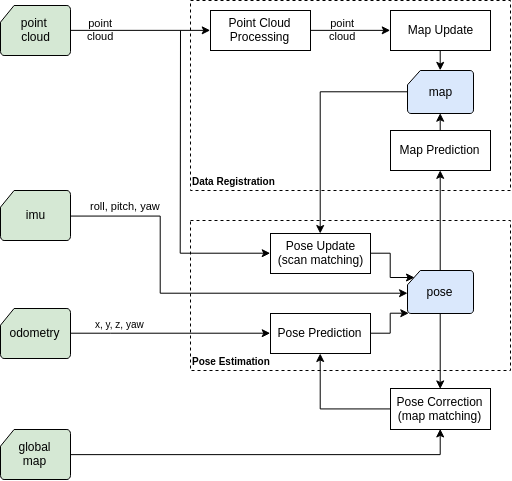
\includegraphics[scale=0.4]{Figures/high_level_design_diagram}
    \decoRule
    \caption[High Level Design Diagram]{
        The high-level design diagram showing the submodules that comprise
        the system as well as the data flow.}
    \label{fig:HLD}
\end{figure}

\section{Data Registration}

An integral aspect of a robotic system, is the mapping process.
The map is the model of the environment and can represent information about
it in either two or three dimensions. In addition, the information a map
represents can be organized either in a grid-based manner (volumetric
map) or in the form of landmarks (feature-based map). Volumetric maps provide
a more detailed and precise model of the environment compared to feature-based
maps and are, therefore, the better choice for robots that aim to solve
navigation tasks. Moreover, autonomous robots that need to navigate in
non-flat surfaces, require a 3D model in order to safely avoid the terrain's
obstacles. Robotic applications with this requirement include outdoor,
underwater, airborne or planetary missions.

% TODO(ref): mapping and classification

As we have already mentioned, planetary rovers have an important constraint
in on-board computational power. This limitation deems the use of pure 3D
maps inappropriate. To overcome this problem, we can represent the
environment with a 2.5D map, known as elevation map. An elevation map
is essentially a 2D grid-map composed of cells that hold the value of
the terrain's elevation. It is important to note that this mapping method
does not model completely the 3D environment, but can provide a
sufficient approximation even for the most demanding applications.

% TODO(ref): elevation map

To make use of this mapping technique, a robot must be equipped with a
sensor that is capable of providing measurements in the 3D space.
Such measurements are usually stored in a structure called point cloud -
a set of points $P$ that contain information about their position in
space $\left(x,y,z\right)$. A point cloud can be constructed from
sensors that provide depth information, with the most popular being stereo
cameras, time-of-flight (ToF) cameras and LiDARs.

% TODO(ref): point cloud

In this section, the functionality of the Data Registration module will be
explained. Its main purpose is to preprocess the input sensor data (point
cloud) and register it to create an elevation map or update an existing one.

\subsection{Point Cloud Preprocessing}

The importance of preprocessing a point cloud before registering its data
in a map, comes from the fact that point clouds contain large amount of points
and hence process them is a time-consuming task. Additionally, the
points represented in the cloud may be referenced in a different frame
(usually the sensor's frame) than the frame of the map.

Explain the processing steps of the input point cloud and why they are needed

\begin{enumerate}
    \item Downsample with voxel grid to have less data (precision trade-off)
    \item Apply TF to bring the points from the sensor frame to the robot frame
    \item Crop to map size to discard out-of-bounds information
    \item Calculate height variance of each point using the sensor's model to create a 1D gaussian
\end{enumerate}

\noindent
Add equations of the sensor model used to calculate the variances\\
Add figure of point cloud pre and post processing

\subsection{Registration}

\subsubsection{Structure of Elevation Map}

Explain the structure of the map and its properties\\
Explain the reference frame of the map with a figure

robot-centric
Map Structure: 4 layers (height gaussian + translation variances)
Map Properties: resolution, length, min/max elevation, 2D position

\subsubsection{Map Prediction and Update}

Explain prediction and update steps

\begin{enumerate}
    \item Prediction
        \begin{enumerate}
            \item Apply delta pose translation (x and y) from particle filter to map
            \item Update translation variances of each cell using translation model
            \item Keep height gaussian of each cell unchanged
        \end{enumerate}
    \item Update
        \begin{enumerate}
            \item Fuse each point of cloud to corresponding map cell by fusing gaussians
            \item Keep translation variances (x and y) of each cell unchanged
        \end{enumerate}
\end{enumerate}

\noindent
Add gaussian fusion equations\\
Add figures of input point cloud and its projection in the map

\section{Data Fusion}

Explain what is the purpose of this step

\begin{itemize}
    \item to get better sensor coverage by fusing multiple sensors
    \item increase map quality using the translation uncertainties
\end{itemize}

\subsection{Sensor Fusion}

Explain how sensor fusion is implemented

\noindent
Mention that calibration errors in sensors as well as inaccuracies in the sensor transformations can cause the sensor fusion to over-smooth obstacles/features causing false negatives

\noindent
Add figures of point clouds from different sensors and the resulting map from fusion

\subsection{Neighborhood Fusion}

Explain what is neighborhood fusion and the steps

\bigskip
\noindent
For each cell of map:
\begin{enumerate}
    \item Compute a weight for every neighboor cell according to distance/variance
    \item Update mean/variance of cell using a weight-based fusion rule
\end{enumerate}

\noindent
Add equation for the weight calculation and the fusion rule\\
If visible, add figures showing the variance layers in the map, and the result of the fusion (prior and posterior mean elevation layers)

\section{Pose Estimation}

Explain what is the purpose of this step
Explain the particle filter used
Explain how IMU measurements are fused to get the final pose

\begin{itemize}
    \item Purpose: to get a better estimate of the pose using the local map
    \item Particle Filter: continuous, estimates 3 states (x, y, yaw) etc.
\end{itemize}

\noindent
Add figure showing the particle distribution around the robot

\subsection{Initialization}

Explain the step

\begin{enumerate}
    \item Sample all particles at initial pose
\end{enumerate}

\noindent
Add gaussian sampling equation

\subsection{Prediction}

Explain the steps

\begin{enumerate}
    \item Add gaussian noise to delta pose transformation from visual odometry
    \item Apply transformation to each particle
\end{enumerate}

\noindent
Add prediction equations (trivial)

\subsection{Update}

Explain the steps

\begin{enumerate}
    \item Crop local map to sensor's dimensions
    \item Create point cloud from local map
    \item Crop raw (input) cloud to map size
    \item Downsample raw and map point clouds (for faster convergence of point cloud alignment)
    \item For each particle
        \begin{enumerate}
            \item Create particle point cloud by transforming map point cloud to particle's pose
            \item Measure particle and raw point cloud alignment using mean square error
            \item Assign inverse error as particle's weight
        \end{enumerate}
\end{enumerate}

\noindent
Add equations of point cloud alignment method for the weight update

\subsection{Resampling}

Explain the technique used, the steps and the strategy

\begin{itemize}
    \item Technique: multinomial resampling
    \item Steps
        \begin{enumerate}
            \item Normalize particle weights to form cummulative distribution
            \item Sample uniformally each particle from cummulative distribution
            \item Strategy: resample every X filter updates, depending on the robot's speed and the particle scattering (noise)
        \end{enumerate}
\end{itemize}

\noindent
Add equations for forming and sampling from the cummulative distribution

\subsection{Estimation}

Explain the steps

\begin{enumerate}
    \item Estimate pose from particle cloud:
        \begin{enumerate}
            \item Ignore particles with weights below a specific threshold
            \item Pick top X particles
            \item Calculate new estimate by performing a weighted average of particles
            \item Calculate pose variance from the distribution of the particle cloud
        \end{enumerate}
    \item Fuse IMU/Odometry states:
        \begin{enumerate}
            \item Get roll and pitch measurements directly from the IMU
            \item Get z estimation directly from visual odometry
            \item Fuse IMU (laser gyroscope) yaw measurement with the PF's yaw estimate by means of 1D gaussian fusion
        \end{enumerate}
\end{enumerate}

\noindent
Add equations for calculating the mean and the variance values of the estimate\\
Mention that the robot's absolute z estimate is not of importance and why is that

\section{Pose Correction}

Explain what is the purpose of this step\\
Explain the execution strategy of this step\\
Mention known limitations of this approach

\begin{itemize}
    \item Purpose: to minimize absolute localization drift using the global map
    \item Strategy:
        \begin{itemize}
            \item Generic: map needs to have features \& robot must have covered certain amount of cells in the global map
            \item Planetary specific: correct pose by the end of the day (for energy efficience reasons)
        \end{itemize}
    \item Limitations:
        \begin{itemize}
            \item When there are no features, the local to global map matching will fail
            \item For safety purposes, the rover tries to generate a global path (using the global map) with as few features (i.e. rocks/craters) as possible
        \end{itemize}
\end{itemize}

\subsection{Global to Local Map Matching}

Explain the steps\\
Explain why a template matching method is used instead of a feature-based one

\begin{enumerate}
    \item Downsample local map to match global map's resolution
    \item Calculate gradient (magnitude of the edge) of local and global map's elevation values
    \item Replace unknown cell values with zero (does not affect matching)
    \item Warp the local map to specific yaw angles to find a yaw correction
    \item For each yaw angle: match local map to global map using template matching with normalized correlation coefficients
 Select or discard best match if score is above X (e.g. 95\%)
    \item Convert the matched position from image coordinates to map coordinates
    \item Add gaussian noise to delta transformation (x \& y) from matching
    \item Apply transformation to each particle of particle filter
\end{enumerate}

\noindent
Add figures of:
\begin{itemize}
    \item comparing Sobel edges with Scharr/Laplacian to justify the method
    \item source global/local maps in the scene (3D)
    \item source global/local maps in 2D
    \item downsampled local map
    \item gradients of global/local maps
    \item result image of matching with rectangles indicating the match \& the ground truth match
\end{itemize}

\noindent
Add equations of:
\begin{itemize}
    \item nearest neighbor method for downsampling the local map
    \item gradient calculations (sobel kernel etc.)
    \item template matching method (normalized correlation coefficients)
    \item selection technique of best position from result image
\end{itemize}

\subsection{Criteria Checking}

\subsubsection{Elevation Features Checking}

Explain the steps and the threshold parameter selection

\begin{enumerate}
    \item Create slope map from local elevation map by calculating the elevation gradient
    \item Remove values in slope map below a specific threshold
    \item Add remaining values to get absolute slope of map
    \item Compare to threshold
\end{enumerate}

\noindent
Add equation for calculating the gradient and thresholding the map (image)\\
Add figures of final slope maps that succeed/fail the criterion

\subsubsection{Traversed Distance Checking}

Explain the step and the threshold parameter selection

\begin{enumerate}
    \item Calculate traversed distance since last pose correction step
    \item Compare to threshold
\end{enumerate}

\noindent
Add equation for the distance calculation (very trivial)\\
Add figures of robot traverses that succeed/fail the criterion

